% ::setlocal makeprg=cd\ report\ &&\ pdflatex\ -interaction=batchmode\ main.tex\ &&\ xdg-open\ main.pdf
% then to compile and open the file just run :make (or press F8)

\documentclass[a4paper, titlepage]{article}
\newcommand{\Punit}[0]{\frac{\unit{\mega\electronvolt}}{c^2 \unit{\femto\cubic\meter}}}
\newcommand{\Sh}[0]{Schwarzschild }

\input{packages}
%\begin{frontespizio}
    \Universita{Trento} % CTT
    \Logo{Figures/logo_unitn} % CTT
    \Divisione{Fisica Computazionale} % CTT
    \Corso[Laurea Triennale]{Fisica} % CTT, a meno che non cambi la denominazione del corso
    \Annoaccademico{2023-2024}
    \Titoletto{Progetto Finale} % CTT
    \Titolo{Calcolo redshift nell'emissione di fotoni da una stella di neutroni\\ }
    \Sottotitolo{\today}
    \Candidato[227552]{Federico De Paoli, \textsf {federico.depaoli@studenti.unitn.it}}
    \NRelatore{Docente}{} % CTT
    \Relatore{Prof. Alessandro Roggero} % CTT, a meno che non sia cambiato il Prof.
\end{frontespizio}
\IfFileExists{\jobname-frn.pdf}{}{%
\immediate\write18{pdflatex \jobname-frn}} % ASSOLUTAMENTE CTT, è il comando che materialmente vi genera il frontespizio.

\newpage



\begin{document}

\tableofcontents
\newpage

\section{Introduzione}
Studiamo la stabilità delle stelle di neutroni in regime relativistico considerando 3 possibili equazioni di stato per la materia.
Una volta risolte le equazioni è possibile ottenere l'espressione del potenziale gravitazione della stella e calcolare l'effetto sulla radiazione emessa dalla stella.


Viene calcolata la radianza per ogni stella a 3 distanze diverse e la potenza totale di emissione in funzione della distanza dalla stella.
Viene quindi calcolata la temperatura apparente delle 3 stelle più massive in funzione di quella effettiva e poi viene studiata la temperatura apparente in funzione della pressione centrale della stella.

\section{Stabilità}

Le equazioni che descrivono la stabilità di una stella in funzione della massa ($m$) e della pressione ($P$) sono quelle di Tolman-Oppenheimer-Volkoff
\begin{subequations}
    \begin{align}[left = {\empheqlbrace}]
        \dv[]{P(r)}{r} &= - G \frac{m(r) \epsilon (r)}{r^2 c^2} \left(1 + \frac{P(r)}{\epsilon (r)} \right) \left(\ + \frac{4 \pi r^3 P(r)}{m(r) c^2} \right) \left(1 - \frac{2 G m(r)}{r c^2} \right)^{-1} \label{eq:P_corr} \\
        \dv[]{m(r)}{r} &= 4 \pi r^2 \frac{\epsilon (r)}{c^2} \label{eq:m_corr} \\
        \dv[]{\Phi(r)}{r} &= - \frac{1}{P(r) + \epsilon (r)} \dv[]{P(r)}{r} \label{eq:Phi_corr}
    \end{align}
    \label{eq:sistema_corr}
\end{subequations}

Dove la terza equazione è l'equazione disaccoppiata e descrive il potenziale gravitazionale della stella.
Usiamo 3 diverse densità di energia per la materia della stella (eq. \ref{eq:energia23} viene presa con due coppie di valori diversi di $\Gamma$ e $K$):
\begin{subequations}
\begin{align}
    \epsilon_1 (n) &= a \left( \frac{n}{n_0} \right) ^{\alpha} + b \left( \frac{n}{n_0} \right) ^{\beta} \label{eq:energia1} \\
    \epsilon_{2/3} (n) &= \mu c^2n+Kc^2n^\Gamma \label{eq:energia23}
\end{align}
\end{subequations}
\begin{equation}
    \text{con} \quad a = 13.4 \unit{\mega\electronvolt\per\femto\cubic\meter} \ , \quad
    \alpha = 0.514, \quad
    b = 5.62 \unit{\mega\electronvolt\per\femto\cubic\meter} \ , \quad
    \beta = 2.436 \ , \quad
    n_0 = 0.16 \unit{\per\femto\cubic\meter}
\end{equation}

dove $n$ è la densità numerica, $\mu$ la massa di una singola particella e quindi $\rho = \mu n$ è la densità di massa.


Visto che la densità di energia è in funzione di $\rho$ e le incognite del sistema \ref{eq:sistema_corr} sono $P$ e $m$ possiamo scrivere la densità di energia in funzione di $P$ e $m$ partendo dalla relazione termodinamica

\begin{subequations}
    \label{eq:eps(r)}
    \begin{align}[left = {P = - \dv[]{E}{V} \Rightarrow \empheqlbrace}]
        P &= (\alpha - 1) a \left( \frac{n}{n_0} \right)^{\alpha} + (\beta - 1) b \left( \frac{n}{n_0} \right)^{\beta} && \text{per } \epsilon_1 \label{eq:eps(r)1} \\
        n &= \left( \frac{P}{K(\Gamma - 1) c^2} \right)^{1 / \Gamma} && \text{per } \epsilon_{1/2} \label{eq:eps(r)23}
    \end{align}
\end{subequations}

Nel primo caso (eq. \ref{eq:eps(r)1}) non è stato possibile invertire l'equazione per trovare $n$ in funzione di $P$ e $m$ quindi utilizzeremo un metodo numerico per trovare $n$ di volta in volta.

Facciamo le seguenti sostituzioni per rendere le variabili adimensionali e con valori più vicini a 0.

\begin{equation*}
    m=M_0\hat m, \quad 
    r=R_0\hat r, \quad 
    P=P_0\hat P, \quad
    \rho=\rho_0 \hat{\rho}, \quad
    K = \hat{K}\frac{\mu^\Gamma}{\rho_0^{\Gamma-1}},
\end{equation*}

\begin{subequations}
    \begin{align}[left = {\empheqlbrace}]
        \dv[]{\hat P}{\hat r} &= - \frac{(\hat P + \hat{\epsilon})(\hat m + \hat r^3 \hat P)}{\hat r^2-2\hat m\hat r} \label{eq:P_ad} \\
        \dv[]{\hat m}{\hat r} &= \hat r^2 \hat{\epsilon} \label{eq:m_ad} \\
        \dv[]{\Phi}{\hat r} &= - \frac{1}{\hat P + \hat{\epsilon}} \dv[]{\hat P}{\hat r} \label{eq:Phi_ad}
    \end{align}
    \label{eq:sistema_adim}
\end{subequations}

Otteniamo il sistema \ref{eq:sistema_adim} dove, grazie alle equazioni in \ref{eq:eps(r)}, $\hat m$, $\hat P$ e $\hat{\epsilon}$ sono funzioni di $\hat r$. Come valori delle costanti sono stati usati

\begin{equation}
    M_0 = 12.655756 M_\odot \quad R_0 = 20.06145 \unit{\kilo\meter} \quad \epsilon = P_0 = \rho_0 c^2 = 150.174 \Punit
    \label{eq:val_cost}
\end{equation}

Per il potenziale gravitazionale $\Phi$ si può inoltre trovare una soluzione analitica all'esterno della stella che possiamo mettere in forma adimensionale (eq. \ref{eq:Phi_ext}), dove $\hat{M}$ e $\hat R$ sono rispettivamente la massa totale e il raggio della stella in forma adimensionale.

\begin{equation}
    \Phi_\text{ext} (r) = \frac{1}{2} \log(1 - \frac{2 G M}{r c^2})
    \implies \Phi_\text{ext} (\hat r) = \frac{1}{2} \log(1 - \frac{2 \hat{M}}{\hat r}) \quad \quad \hat r \geq \hat{R}
    \label{eq:Phi_ext}
\end{equation}


\section{Curva massa raggio}
Cominciamo con il risolvere le prime due equazioni \ref{eq:P_ad} e \ref{eq:m_ad} del sistema adimensionale con il metodo \texttt{RK4} (appendice \ref{ap:RK4}).
Per il caso con equzione di stato più complessa (eq. \ref{eq:energia1}) viene risolta numericamente l'equazione \ref{eq:eps(r)1} per trovare $\rho$ da $P$ (Appendice \ref{ap:eps(r)1}).

Segliamo massa iniziale 0 e pressioni iniziali differenti in modo da trovare soluzioni con $R$ compreso tra i 3 e i 60 \unit{\kilo\meter}. Il grafico massa raggio trovato viene riportato in figura \ref{fig:MR}.

\begin{figure}[h]
        \centering
        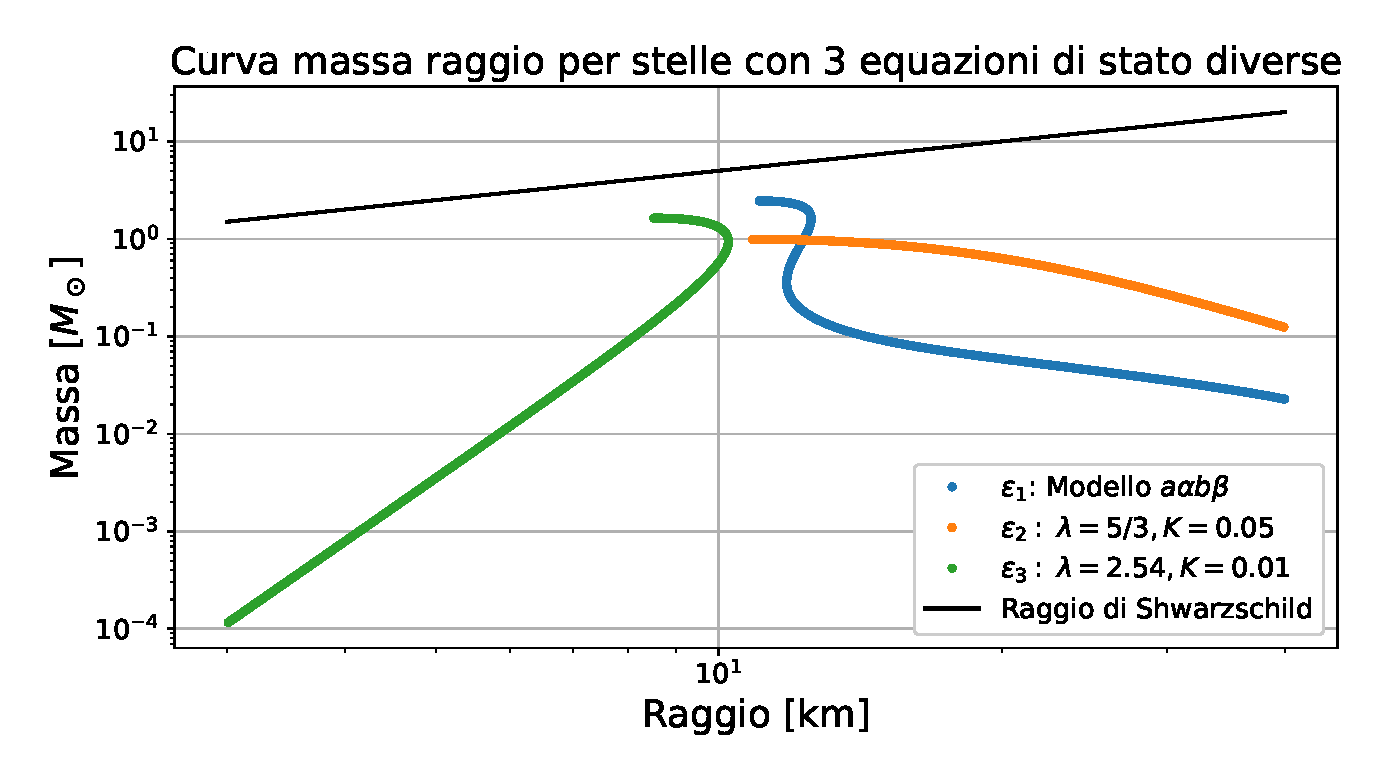
\includegraphics[width = 0.6 \textwidth]{Figures/MR.eps}
        \caption{Curva massa raggio per stelle di equzioni di stato $\epsilon_{1/2/3}$. La prima equazione di stato, quella più realistica, prevede stelle di neutroni più massive.}
        \label{fig:MR}
\end{figure}

Durante l'esecuzione del programma abbiamo inoltre smesso di incrementare la pressione centrale iniziale quando la condizione di stabilità $\dv[]{M}{r} > 0$ veniva meno.

Notiamo subito che con l'equazione di stato \ref{eq:energia1} il modello prevede stelle con massa e raggio maggiore rispetto al limite previsto dagli altri modelli.

I valori della stella più massiva per ogni equazione di stato diversa vengono riportati nella tabella \ref{tab:Mgrosso}.

\begin{table}[h!]
    \centering
    \begin{tabular}{c|c|c|c}
        & $P_0~[\Punit]$ & $R~[\unit{\kilo\meter}]$ & $M~[M_\odot]$ \\
         \hline
         $\epsilon_1$ & 43.31065 & 59.03824 & 14.29963 \\
         \hline
         $\epsilon_2$ & 217.0675 & 10.90280 & 0.9252994 \\
         \hline
         $\epsilon_3$ & 947.5339 & 8.559218 & 1.528782 \\
    \end{tabular}
    \caption{Valori della pressione iniziale $P_0$, massa totale $M$ e raggio $R$ della stella più massiva per ogni equazione di stato utilizzata.}
    \label{tab:Mgrosso}
\end{table}


\section{Potenziale gravitazionale}

Come mostrato nel sistema \ref{eq:sistema_corr}, l'equzione che determina il potenziale gravitazionale è disaccoppiata dalle altre due e, per $r \geq R$, può anche essere risolta analiticamente.
Utilizzando le equazioni \ref{eq:Phi_ad} e \ref{eq:Phi_ext} possiamo trovare l'espressione generale per il potenziale all'interno della stella riportata in eq. \ref{eq:Phi_int1}.

\begin{equation}
    \Phi_\text{int} (\hat r) =
    \Phi_\text{ext} (\hat R) - \int_{\hat r}^{\hat R} \dv[]{\Phi}{x} \;\mathrm{d}x =
    \frac{1}{2} \log(1 - \frac{2 \hat M}{\hat R}) + \int_{\hat r}^{\hat R} \frac{1}{\hat P (x) + \hat \epsilon (x)} \dv[]{\hat P (x)}{x} \;\mathrm{d}x
    \label{eq:Phi_int1}
\end{equation}

dove siamo stati attenti a rendere $\Phi (r)$ continuo per ogni $r \geq 0$ usando il valore di $\Phi_\text{ext}$ in $\hat R$. Infine sostituendo alla derivata della pressione l'espressione in \ref{eq:P_ad} otteniamo

\begin{equation}
    \Phi_\text{int} (\hat r) =
    \frac{1}{2} \log(1 - \frac{2 \hat{M}}{\hat R}) + \int_{\hat r}^{\hat R} \frac{\hat m (x) + x^3 \hat P (x)}{2 \hat m (x) x - x^2}  \;\mathrm{d}x
    \label{eq:Phi_int2}
\end{equation}

Dati i valori di $\hat P (\hat r)$ e $\hat m (\hat r)$ che si ottengono risolvendo le equazioni di stabilità possiamo quindi risolvere l'integrale con il metodo dei trapezi per ottenere il valore di $Phi$ a ogni $r$ (Appendice \ref{ap:Phi}). Il grafico del potenziale gravitazionale ottenuto è mostrato in figura \ref{fig:Phi}.

\begin{figure}[h]
    \centering
    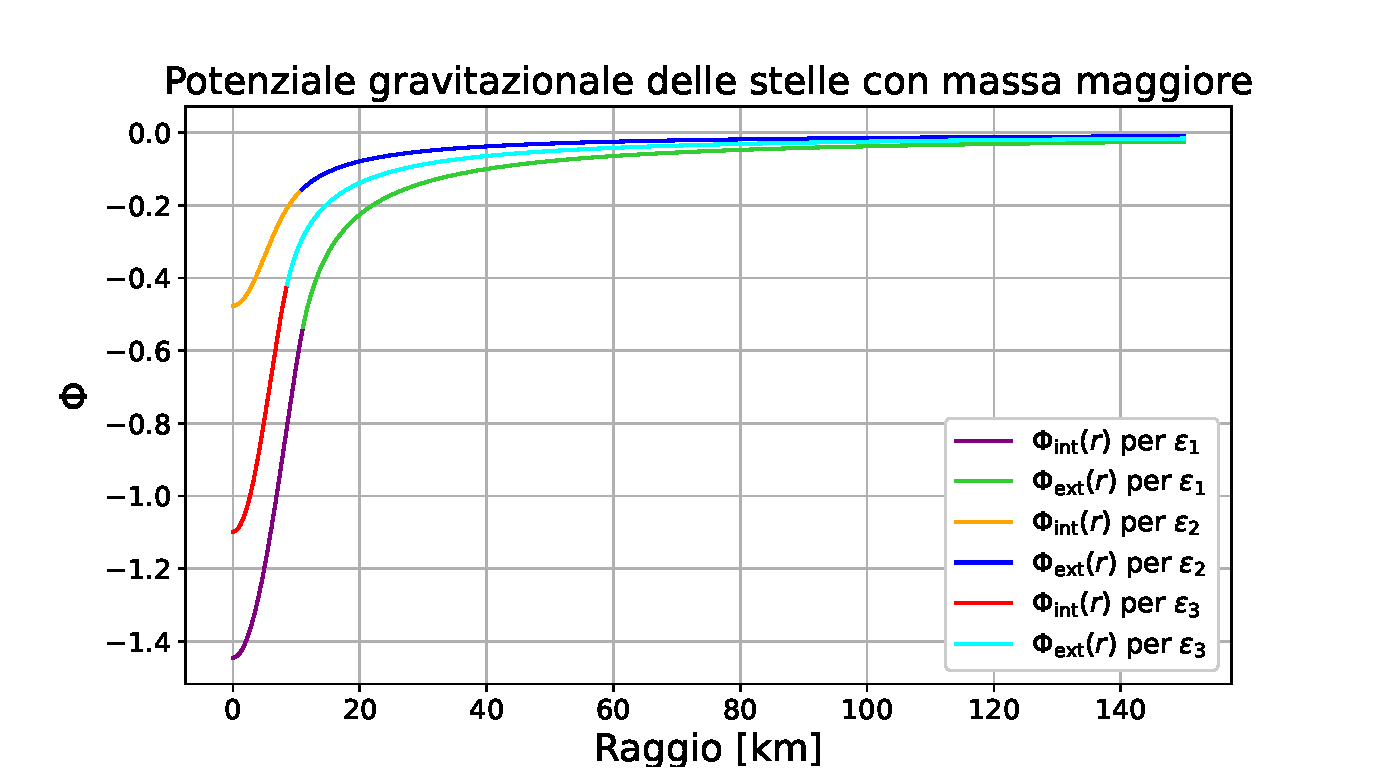
\includegraphics[width = \textwidth]{Figures/Phi.eps}
    \caption{Grafico del potenziale gravitazionale all'interno e all'esterno della stella. Per $r < R$ è stato ottenuto integrando con il metodo dei trapezi l'eq. \ref{eq:Phi_int2}, per $r \geq R$ è stata plottata l'eq. \ref{eq:Phi_ext}}
    \label{fig:Phi}
\end{figure}

Vediamo dalla figura \ref{fig:Phi} che in tutti e 3 i casi $\Phi (r)$ è continuo, grazie alla condizione imposta.

Il potenziale $\Phi$ (che fa parte del termine $e^{\Phi (r)} c^2 \mathrm{d}t^2$ della metrica $\mathrm{d}s^2$, che descrive la geometria dello spazio vicino alla stella) assume un andamento famigliare: raggiunge valori più bassi per le stelle più massive al diminuire di $r$ e tende a 0 per $r$ grandi.



\section{Radianza} \label{sec:rad}

In metrica di \Sh un fotone emesso a distanza $r$ con frequenza $\nu_\text{em}$ viene ricevuto da un osservatore a distanza $r'$ con una frequeza $\nu_\text{ric}$ data da

\begin{equation}
    \frac{\nu_\text{ric}}{\nu_\text{em}} = e^{\Phi (r) - \Phi (r')} \, .
\label{eq:redshift}
\end{equation}

Dove $\Phi (r)$ è propio il potenziale gravitazionale mostrato in figura \ref{fig:Phi}.

La radianza di una stella si può esprimere con l'equazione di Plank per il corpo nero

\begin{equation}
    B(\nu, T) = \frac{2 h \nu ^3}{c^2} \frac{1}{e^{h \nu / (k_B T)} - 1}
    \label{eq:rad}
\end{equation}

dove $T$ è la temperatura della stella e $h$ la costante di Plank.
Per fare i conti considerando solo il caso con $K_B T = 1 \unit{\mega\electronvolt}$ e mettiamo l'equzione \ref{eq:rad} in funzione di variabili adimensionali. Otteniamo

\begin{equation*}
    \hat B(\hat \nu) = \frac{\hat \nu ^3 }{e^{\hat \nu} - 1}
    \label{eq:rad_ad}
\end{equation*}
dove abbiamo definito
\begin{align*}
    \nu_0 &= \frac{\nu}{\hat \nu} = \frac{h}{1\unit{\mega\electronvolt}} \simeq \num{2.417989e20} \unit{\hertz} \\
    B_0 &= \frac{B}{\hat B} = \frac{2 h \nu_0^3}{c^2} = \frac{2 \unit{\mega\electronvolt}}{(h c)^2} \simeq \num{1.301059e-6} \frac{\unit{\mega\electronvolt}}{\unit{\femto\meter\squared}}
\end{align*}

Infine, se consideriamo l'effetto doppler dovuto al potenziale gravitazionale descritto in eq. \ref{eq:redshift} e utilizziamo la formula analitica per il potenziale gravitazionale all'esterno della stella (eq. \ref{eq:Phi_ext}), otteniamo

\begin{equation}
    \hat \nu_\text{em} = \hat \nu_\text{ric} \left ( \frac{1 - \frac{2 \hat M}{r}}{1 - \frac{2 \hat M}{\hat R}}\right )^{1/2}
    \quad
    \implies
    \quad
    \hat B(\hat \nu_\text{ric}, \hat r) =
    \frac{\hat \nu_\text{ric}^3 \left(1 - \frac{2 \hat M}{\hat r}\right)^{3/2} \left(1 - \frac{2 \hat M}{\hat R}\right)^{-3/2} }
    {\exp( \hat \nu_\text{ric} \left(1 - \frac{2 \hat M}{\hat r} \right)^{1/2} \left(1 - \frac{2 \hat M}{\hat R}\right)^{-1/2} ) - 1}
    \label{eq:B_corr}
\end{equation}

Nel figure \ref{fig:rad1}, \ref{fig:rad2} e \ref{fig:rad3} viene studiato lo spettro della radiazione emessa per le 3 stelle massive di cui abbiamo studiato il potenziale in \ref{fig:Phi} a distanze diverse dalla stella.
In blu è plottata l'eq. \ref{eq:rad}, ovvero la radianza senza correzioni relativistiche.

\begin{figure}[h]
    \begin{minipage}{0.49\textwidth}
        \centering
        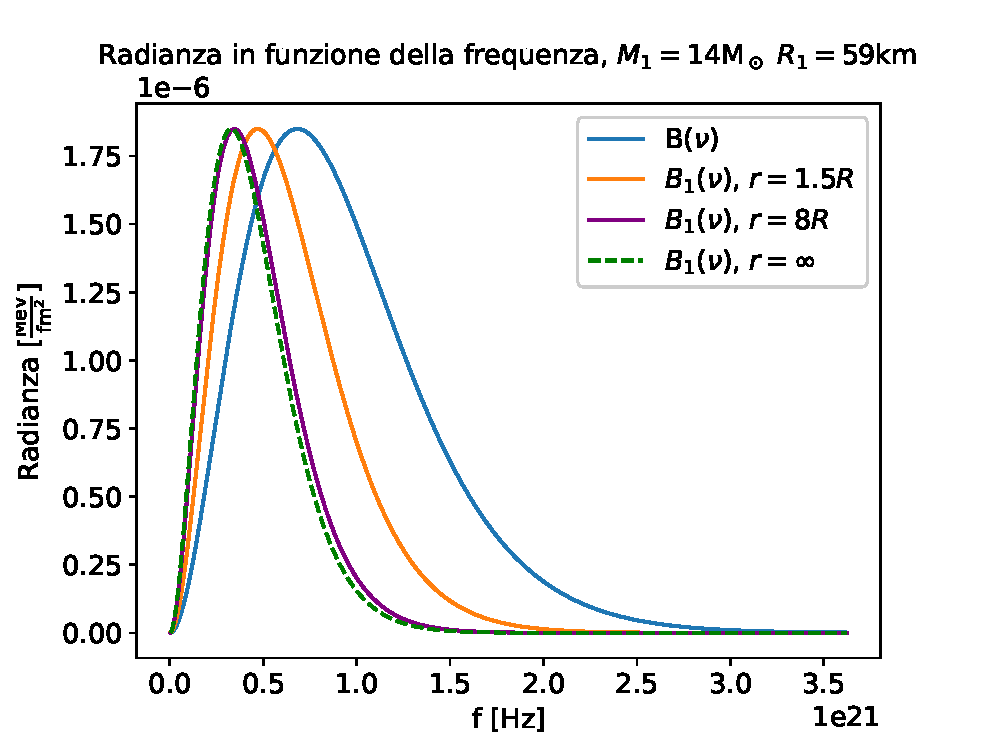
\includegraphics[width = \textwidth]{Figures/radianza1.eps}
        \caption{Radianza di una stella con $M = 14M_\odot$ e $R = 59\unit{\kilo\meter}$, percepita a $88.6 \unit{\kilo\meter}$, $472 \unit{\kilo\meter}$ e a distanza infinita.
        Essendo la stella con massa maggiore è anche quella in cui il redshift è più visibile.}
        \label{fig:rad1}
    \end{minipage}
    \hspace{0.015\textwidth}    
    \begin{minipage}{0.49\textwidth}
        \centering
        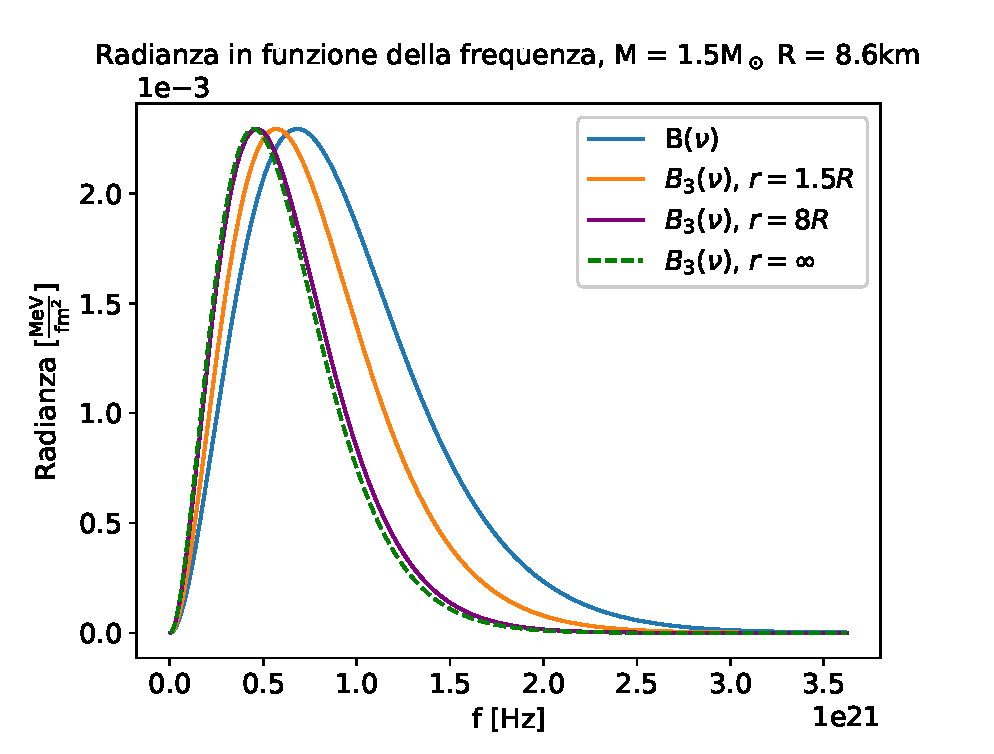
\includegraphics[width = \textwidth]{Figures/radianza3.eps}
        \caption{Radianza da una stella con $M = 1.5M_\odot$ e $R = 8.6\unit{\kilo\meter}$, percepita a $12.8 \unit{\kilo\meter}$, $68.5 \unit{\kilo\meter}$ e a distanza infinita.
        In blu la radianza senza correzioni relativistiche.\\}
        \label{fig:rad2}
    \end{minipage}
\end{figure}

La curva in tutti e 3 i casi subisce uno spostamento verso le frequenze più basse, \textit{redshift} per l'appunto, e l'effetto è tanto maggiore quanto più la stella è massiva e l'osservatore distante. Già a una distanza di 8 volte il raggio della stella la curva della radianza è molto simile a quella all'inifinito, in cui il termine $\Phi (r')$ in eq. \ref{eq:redshift} è trascurabile.
\begin{figure}[h]
    \centering
    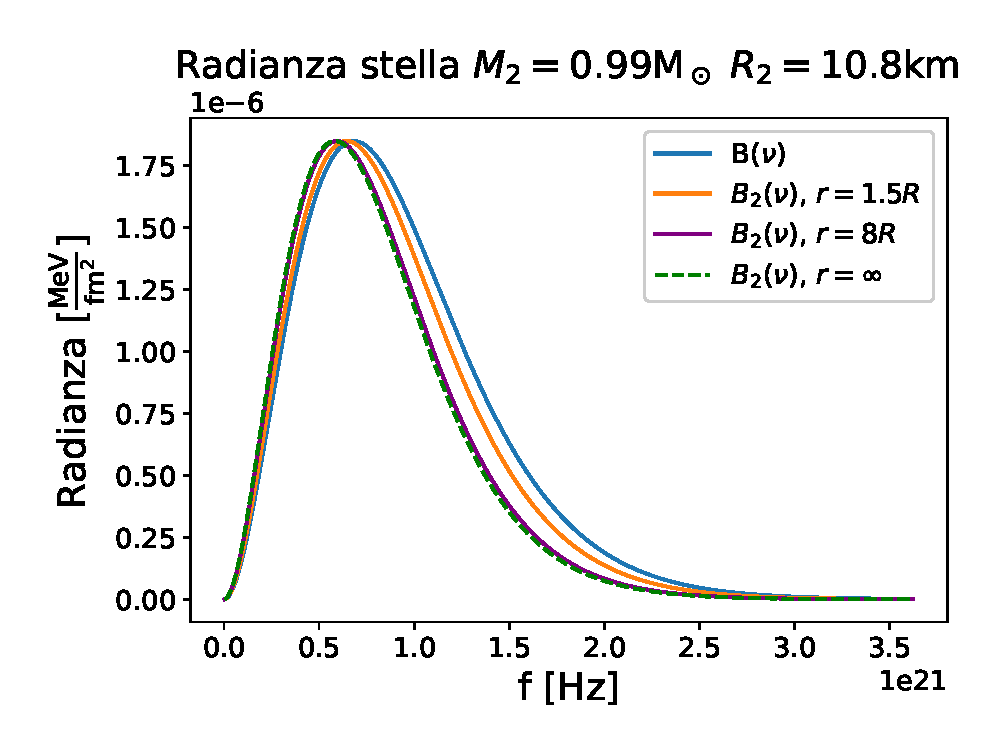
\includegraphics[width = 0.6 \textwidth]{Figures/radianza2.eps}
    \caption{Radianza da una stella con $M = 0.93M_\odot$ e $R = 11\unit{\kilo\meter}$, percepita a 16.4, 87.2 \unit{\kilo\meter} e a distanza infinita.
    In blu la radianza senza correzioni relativistiche.}
    \label{fig:rad3}
\end{figure}



\section{Potenza emessa}

La potenza totale emessa dalla stella, per unità di area, si può ottenere integrando la radianza $B(\nu, T)$ sulle frequenze e sulla superficie della sfera centrata nella stella, eq. \ref{eq:Pot}.

\begin{equation}
    \mathcal P = \int_0^\infty \; \mathrm{d}\nu \int B(\nu, T) \cos(\theta) \; \mathrm{d}\Omega
    = 4 \pi \int_0^{A k_B T} B(\nu, T) \; \mathrm{d}\nu
    \label{eq:Pot}
\end{equation}

Utilizzando la stessa temperatura della sezione \ref{sec:rad}, $k_B T = 1 \unit{\mega\electronvolt}$, e le unità adimensionali, l'integrale in \ref{eq:Pot} può essere riscritto come

\begin{equation}
    \hat{\mathcal P}(\hat r) = \int_o^{\frac{A \unit{\mega\electronvolt}}{\nu_0}} \hat B (\hat \nu_\text{ric}, \hat r) \; \mathrm{d} \hat \nu
    \label{eq:Pot_ad}
\end{equation}

dove $\hat B (\hat \nu_\text{ric}, \hat r)$ è definita in \ref{eq:B_corr} e

\begin{equation}
    \mathcal P_0 = \frac{\mathcal P}{\hat {\mathcal P}} = 2 \pi B_0 \nu_0 \simeq \num{1.976658e+15} \, \frac{\unit{\mega\electronvolt}}{\unit{\second\femto\meter\squared}}
\end{equation}

Dal momento che numericamente non è possibile integrare sulle frequenze fino a $\nu = + \infty$ si sceglie $A$ sufficientemente grande da poter approssimare in modo ragionevole l'integrale.
Facendo riferimento alla figura \ref{fig:rad2}, possiamo vedere che per $\nu > \num{3.5e21} \unit{\hertz}$ la radianza è quasi nulla.
In quell'occasione era stata calcolata $\hat B(\hat \nu)$ tra $0$ e $15$. Come stima iniziale possiamo quindi integrare fino a $\hat \nu = 20$ che corrisponde a

\begin{equation}
    \frac{A \unit{\mega\electronvolt}}{\nu_0} = 20
    \quad \iff \quad
    A = 20 \nu_0 \unit{\per\mega\electronvolt} \simeq \num{4.835978} \, \unit{\per\second\per\mega\electronvolt}
    \label{eq:A}
\end{equation}

Possiamo ottenere un valore migliore valutando la convergenza dell'integrale. Per prima cosa verifichiamo per quale \texttt{N} (numero di step nell'integrazione) il valore di $\mathcal{P}$ converge (il codice si trova in Appendice \ref{ap:integrali}).

Utilizzando una delle stelle come esempio, a una distanza $r = 1.5R_1 = 86.6 \unit{\kilo\meter}$ e con $\hat \nu_\text{max} = 20$ otteniamo il grafico in figura \ref{fig:Pot_cvgN}. I valori sono degli scarti rispetto a $\mathcal{P}_{N = 1e7}$ (la potenza calcolata con $N = \num{1e7}$) e sono normalizzati rispetto alla stessa.
Come ci aspettavamo io metodo simpson converge più velocemente dei trapezi (e con un costo computazionale maggiore), per entrambi i metodi comunque $\texttt{N} = \num{1e3}$ in un intervallo $\Delta \hat \nu = 20$ è più che sufficienti per garantire una precisione di $\num{1e-8}$.
\begin{figure}[h]
    \begin{minipage}{0.49 \textwidth}
        \centering
        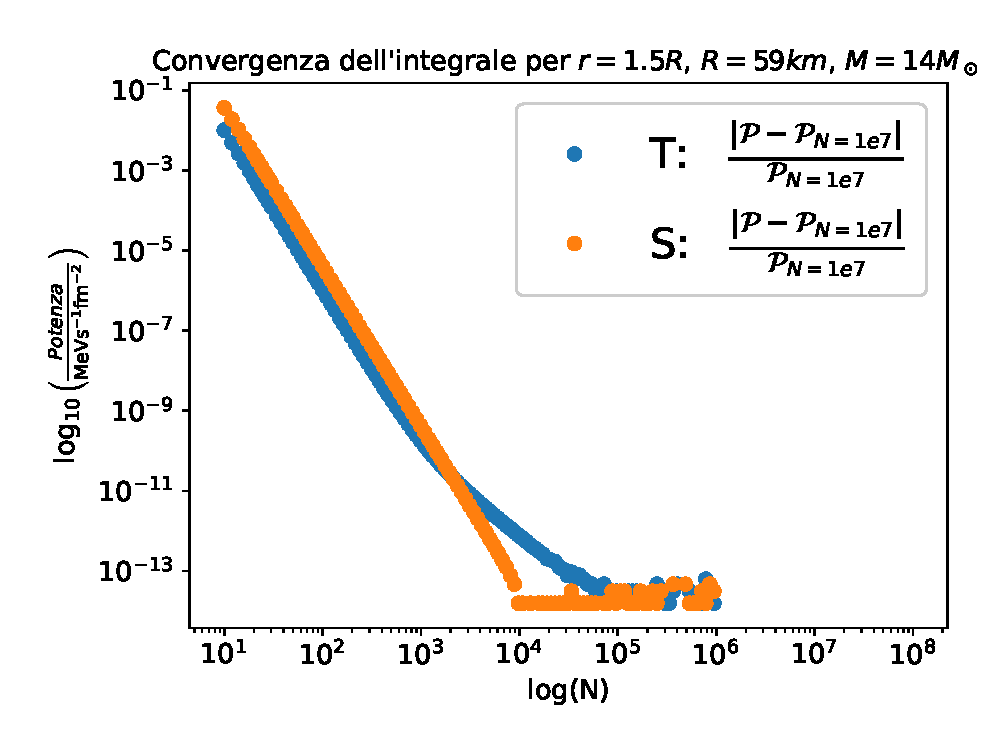
\includegraphics[width = \textwidth]{Figures/Pot_cvgN.eps}
        \caption{Errore relativo sul calcolo della potenza per diversi \texttt{N} (numero di step nell'integrazione con i trapezi \textbf{T} e con simpson \textbf{S}). Per $N > \num{1e3}$ otteniamo una precisione maggiore di \num{1e-8}.}
        \label{fig:Pot_cvgN}
    \end{minipage}
    \hspace{0.01 \textwidth}
    \begin{minipage}{0.49 \textwidth}
        \centering
        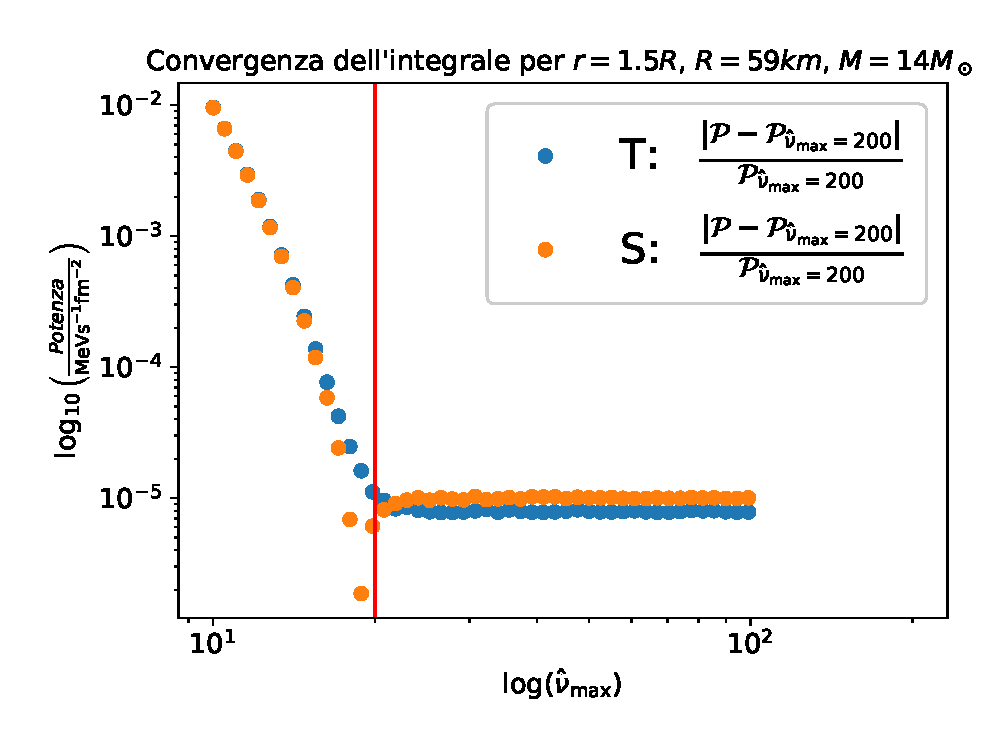
\includegraphics[width = \textwidth]{Figures/Pot_cvgA.eps}
        \caption{Errore relativo sul calcolo della potenza per diversi valori di $\hat \nu_\text{max}$.
        Per $\hat \nu_\text{max} > \num{20}$ (line verticale rossa) otteniamo una precisione maggiore di \num{1e-8}, il valore di A trovato in \ref{eq:A} è quindi una buon upperboud.}
        \label{fig:Pot_cvgA}
    \end{minipage}
\end{figure}

Fissato $\texttt{N} = \num{1e3}$ per un intervallo $\Delta \hat \nu = 20$ proponiamo quindi in figura \ref{fig:Pot_cvgA} lo stesso tipo di grafico degli scarti fatto però in funzione della scelta di $\nu_\text{max}$, questa volta viene utilizzato solo il metodo dei trapezi in quanto è irrilevante.

Alla luce del grafico la scelta di $\hat \nu_\text{max} = 20$ e quindi $A \simeq \num{4.835978} \, \unit{\per\second\per\mega\electronvolt}$ si rivela sufficentemente buona.











%%%%%%%%%%%%%%%%%%%%%%%%%%%%%%%%%%%%%%%%%%%%%%%%%%%%%%%%%%%%%%%%%%%%%%%%%%%%%%%%%%%%%%%%%
%%%%%%%%%%%%%%%%%%%%%%%%                APPENDICI               %%%%%%%%%%%%%%%%%%%%%%%%% 
%%%%%%%%%%%%%%%%%%%%%%%%%%%%%%%%%%%%%%%%%%%%%%%%%%%%%%%%%%%%%%%%%%%%%%%%%%%%%%%%%%%%%%%%%

\newpage
\appendix

\section{RK4} \label{ap:RK4}
Codice con cui è stato implementato il metodo \texttt{RK4}. \texttt{fun\_P()} e \texttt{fun\_m()} sono le funzioni presenti a destra dell'uguale nella prima e nella seconda riga del sistema \ref{eq:sistema_adim}.

\begin{lstlisting}[language=C]
void rungeKutta4(double h, double r, double *P, double *m, int tipo_politropica){

    double k1, k2, k3, k4, l1, l2, l3, l4;

    k1 = h * fun_m(r, *P, tipo_politropica);
    l1 = h * fun_P(r, *P, *m, tipo_politropica);

    k2 = h * fun_m(r + h / 2, *P + l1 / 2, tipo_politropica);
    l2 = h * fun_P(r + h / 2, *P + l1 / 2, *m + k1 / 2, tipo_politropica);

    k3 = h * fun_m(r + h / 2, *P + l2 / 2, tipo_politropica);
    l3 = h * fun_P(r + h / 2, *P + l2 / 2, *m + k2 / 2, tipo_politropica);

    k4 = h * fun_m(r + h, *P + l3, tipo_politropica);
    l4 = h * fun_P(r + h, *P + l3, *m + k3, tipo_politropica);

    *m += (k1 + 2 * k2 + 2 * k3 + k4) / 6;
    *P += (l1 + 2 * l2 + 2 * l3 + l4) / 6;
}
\end{lstlisting}



\section{Risoluzione numerica di $\hat P (\rho)$} \label{ap:eps(r)1}

Quando si calcola il valore della derivata di $P$ o $m$ ad un dato $r$ serve anche il valore dell'energia interna, infatti
\begin{lstlisting}[language=C]
// fun_m = r^3 E
double fun_m(double r, double P, int tipo_politropica){
    return r * r * fun_E(P, tipo_politropica);
}


// fun_P = - (P + E)(m + r^3 P)/(r^2 - 2mr)
double fun_P(double r, double P, double m, int tipo_politropica){
    if (m == 0)
        return 0;
    return (P + fun_E(P, tipo_politropica)) * (m + pow(r, 3) * P) / ((2 * m - r) * r);
}
\end{lstlisting}
Dove la funzione \texttt{fun\_E()} è definita come
\begin{lstlisting}[language=C]
double fun_E(double P, int tipo_politropica){
    // Politropica quasi realistica (a*rho^alpha + b*rho^beta)
    if (tipo_politropica == 0){
        double rho = findRho(P);
        return A * pow(rho, ALPHA) + B * pow(rho, BETA);
    }

    double lambda, K;

    // Politropiche semplici
    if (tipo_politropica == 1){
        lambda = 5. / 3.;
        K = 0.05;
    } else if (tipo_politropica == 2){
        lambda = 2.54;
        K = 0.01;
    } else {
        printf("Tipo politropica non riconosciuto\n");
        return 0;
    }

    double a1 = P / (lambda - 1);
    return a1 + pow(a1 / K, 1. / lambda);
}
\end{lstlisting}

Per le politropiche semplici (eq. \ref{eq:energia23}) abbiamo potuto trovare un'espressione analitica per $\rho (P)$ (eq. \ref{eq:eps(r)23}). L'energia può quindi essere calcolata in modo diretto come viene fatto nelle righe 22-23 del codice sopra riportato.

Per la politropica \ref{eq:energia1}, la relazione tra $\rho$ e $P$ che si trova è data in \ref{eq:eps(r)1}, che riportiamo

\begin{equation}
        P = (\alpha - 1) a \left( \frac{n}{n_0} \right)^{\alpha} + (\beta - 1) b \left( \frac{n}{n_0} \right)^{\beta} \ .
        \label{ap:eq:1}
\end{equation}

Data una certa pressione $P$ bisopgna quindi risolvere numericamente l'equazione per trovare il valore $n$ che la soddisfa. Per fare ciò utiliziamo la funzione \texttt{findRho()} così definita

\begin{lstlisting}[language=C]
double findRho(double P){

    // Cominciamo prima con il metodo di Newton-Raphson
    if (P > 0.01){

        double rho = pow(P / (BETA1 * B), 1 / BETA);    // buona approx. iniziale
        while (fabs(P - P_of_rho(rho)) > 1e-6){
            rho -= (P_of_rho(rho) - P) / DP_of_rho(rho);
        }
        return rho;
    }

    // Per P piccoli meglio usare bisezione
    double rho_sx = 0.7, rho_dx = 1.;
    double rho = (rho_sx + rho_dx) / 2;
    while (fabs(P - P_of_rho(rho)) > 1e-6){
        if (P_of_rho(rho) > P)
            rho_dx = rho;
        else
            rho_sx = rho;
        rho = (rho_sx + rho_dx) / 2;
    }
    return rho;
}
\end{lstlisting}

dove \texttt{P\_odf\_rho()} e \texttt{DP\_of\_rho()} sono rispettivamente la funzione \ref{ap:eq:1} e la sua derivata. In questo modo possiamo sempre trasformare $\epsilon (\rho)$ in $\epsilon (P)$.



\section{Risoluzione dell'integrale del potenziale gravitazionale} \label{ap:Phi}

Per ognuna delle 3 stelle trovate (la più massiva per ogni diversa equazione di stato) salviamo ogni valore di $r$, $m$ e $P$ in un file che successivamente importiamo (riga 3) e utiliziamo per calcolare l'integrale

\begin{lstlisting}[language=C]
double r[lenfile], P[lenfile], m[lenfile], Phi[lenfile];

read_maxM_data(tipo_politropica, lenfile, r, P, m);

double R = r[lenfile - 1];
double M = m[lenfile - 1];
double Phi_ext = fun_Phi_ext(R, M);
double integral = 0;
double h = 1e-5;

// Partiamo a calcolare Phi dalla fine (r = R) perche' e' quando l'integrale e' piu' piccolo
for (int i = lenfile - 1; i > 0; i--){
    integral += h / 2 * (fun_to_integrate(r[i], m[i], P[i]) + fun_to_integrate(r[i - 1], m[i - 1], P[i - 1]));
    Phi[i] = Phi_ext + integral;
}

char Phi_int_filename[50];
sprintf(Phi_int_filename, "../data/Phi_int_%d.csv", tipo_politropica);
FILE *f_Phi_int = fopen(Phi_int_filename, "w");
fprintf(f_Phi_int, "r,Phi\n");
for (int i = 0; i < lenfile; i++)
    fprintf(f_Phi_int, "%.10e,%.10e\n", r[i] * R0, Phi[i]);
fclose(f_Phi_int);

// Calcoliamo anche Phi_ext(r) per r > R
double r_ext = R;

char Phi_ext_filename[50];
sprintf(Phi_ext_filename, "../data/Phi_ext_%d.csv", tipo_politropica);
FILE *f_Phi_ext = fopen(Phi_ext_filename, "w");
fprintf(f_Phi_ext, "r,Phi\n");

while (r_ext < 150 / R0){
// for (int i = 0; i < lenfile; i++){
    fprintf(f_Phi_ext, "%.10e,%.10e\n", r_ext * R0, fun_Phi_ext(r_ext, M));
    r_ext += h;
}

fclose(f_Phi_ext);
\end{lstlisting}

L'integrale (calcolato esplicitamente nella riga 13) può essere valutato solo nei punti $r$ che sono stati utilizzati durante la risoluzione delle equazioni di stabilità della stella.

Per ottimizzare il codice, invece che calcolare l'intero integrale per ogni punto $r$ del grafico di $\Phi(r)$, partiamo da $r = R$ (ovvero quando l'integrale è nullo) e aggiungiamo il valore di 1 trapezio per volta alla variabile \texttt{integral}. In contemporanea, durante una iterazione del ciclo \texttt{for} possiamo utilizzare il valore (parziale) di \texttt{integral} per calcolare $\Phi_\text{int}$ in $r$.

Infine dalla riga 25 calcoliamo $\Phi_\text{ext}$ utilizzando la funzione analitica.



\section{Integrali con trapezi e simpson} \label{ap:integrali}

Le funzioni che fanno l'integrale con i due metodi sono

\begin{lstlisting}[language=C]
// Metodo Trapezi
double integrale_trapezio(double a, double b, int N, double r, double R, double M, double (*fun)(double, double, double, double)){
    // assume a < b
    double h = (b - a)/ (double)N;
    double integral = ((*fun)(a, r, R, M) + (*fun)(b, r, R, M)) * h / 2;

    for (int i = 1; i < N; i++) {
    integral += h * (*fun)(a + i * h, r, R, M);
    }


    return integral;
}

// Metodo Simpson
double integrale_simpson(double a, double b, int N, double r, double R, double M, double (*fun)(double, double, double, double)){
    // assume a > b
    double h = (b - a)/N;
    double integral = ((*fun)(a, r, R, M) + (*fun)(b, r, R, M)) * h / 3;

    // assume N pari
    for (int i = 1; i <= N/2 - 1; i++) {
        integral += (2 * h /3) * (*fun)(a + 2 * i * h, r, R, M);
        integral += (4 * h / 3) * (*fun)(a + (2 * i - 1) * h, r, R, M);
    }


    integral += (4 * h / 3 ) * (*fun)(a + (N - 1) * h, r, R, M);

    return integral;
}
\end{lstlisting}

e per controllare la convergenza del valore della potenza usiamo

\begin{lstlisting}[language=C]
double R[3] = {59.03824 / R0, 10.90280 / R0, 8.559218 / R0};
double M[3] = {14.29963 / M0, 0.9252994 / M0, 1.528782 / M0};
double r[3] = {1.5, 8., -1};
int N = 10;
double Pot, nu_max = 20.;

// Test cvg per N trapezi
FILE *f0 = fopen("../data/potenza/test_cvg_N_trap.csv", "w");
fprintf(f0, "Pot,N,nu_max\n");
while(N <= 1e6){
    Pot = integrale_trapezio(1e-10, nu_max, N, r[0] * R[0], R[0], M[0], &funB_corrected);
    fprintf(f0, "%.13e,%d,%.13e\n", Pot * POT0, N, nu_max * nu0);
    N *= 1.1;
}
fclose(f0);

N = 10;

// Test cvg per N simpson
FILE *f1 = fopen("../data/potenza/test_cvg_N_simp.csv", "w");
fprintf(f1, "Pot,N,nu_max\n");
while(2 * N <= 1e6){
    Pot = integrale_simpson(1e-10, nu_max, 2 * N, r[0] * R[0], R[0], M[0], &funB_corrected);
    fprintf(f1, "%.13e,%d,%.13e\n", Pot * POT0, N, nu_max * nu0);
    N *= 1.1;
}
fclose(f1);

// Come N va bene
N = 1e3;
// Test cvg per nu_max (A)
nu_max = 10;
int Nrel = (double)N / nu_max;
// Test cvg per A (ovvero nu_max)
FILE *f2 = fopen("../data/potenza/test_cvg_A_trap.csv", "w");
fprintf(f2, "Pot,N,nu_max[ad]\n");
while(nu_max <= 1e2){
    N = Nrel * nu_max;
    Pot = integrale_trapezio(1e-10, nu_max, N, r[0] * R[0], R[0], M[0], &funB_corrected);
    fprintf(f2, "%.13e,%d,%.13e\n", Pot * POT0, N, nu_max);
    nu_max *= 1.1;
}
fclose(f2);
\end{lstlisting}

\end{document}



































%% Snippets cos I'm too lazy to set the Lsp the right way


%\begin{figure}[h]
%    \begin{minipage}{0.48\textwidth}
%        \centering
%        \includegraphics[width = \textwidth]{Figures/Figure_rho0.91.png}
%        \caption{Coordinate x e y delle particelle.
%        Sullla stessa fiura sono state plottate le posizioni delle particelle per ogni instante temporale successivo a \texttt{nsteps/2} e per ogni valore di $z$.
%        A $\rho = 0.91$ le particelle sono disposte in modo disordinato. \\}
%        \label{fig:rho0.91}
%    \end{minipage}
%    \hspace{0.015\textwidth}    
%    \begin{minipage}{0.48\textwidth}
%        \centering
%        \includegraphics[width = \linewidth]{Figures/Figure_rho0.97.png}
%        \caption{Coordinate x e y delle particelle.
%        Sullla stessa fiura sono state plottate le posizioni delle particelle per ogni instante temporale successivo a \texttt{nsteps/2} e per ogni valore di $z$.
%        A $\rho = 0.97$ la struttura \texttt{BCC} è ben visibile e per ogni posizione si vede quanto può oscillare una particelle.}
%        \label{fig:rho0.97}
%    \end{minipage}
%\end{figure}


%\begin{table}[h!]
%    \centering
%    \begin{tabular}{c|c|c|c}
%          & SC & BCC & FCC \\
%         \hline
%         $N$ & $n^3$ & $2 n^3$ & $4 n^3$ \\
%         \hline
%         $a$ & $\rho^{-1/3}$ & $\left( \frac{\rho}{2} \right)^{-1/3}$ & $\left( \frac{\rho}{4} \right)^{-1/3}$ \\
%    \end{tabular}
%    \caption{Dipendenza di $N$ e $a$ da $n$ e $\rho$}
%    \label{tab:my_label}
%\end{table}
